數據顯示用在航太工業的碳纖維複合材料上面的鑽孔洞,偏離名義直徑的資料。表中描述偏離名義直徑的數值,數值是以英吋小數點以下萬分位表示。(data: Exercise)
\begin{lstlisting}[language=R]
> data_2 <- read.csv("/Users/pao/Downloads/Exercise.csv")
> data_2
   Sample  x1  x2  x3  x4  x5
1       1 -30  50 -20  10  30
2       2   0  50 -60 -20  30
3       3 -50  10  20  30  20
4       4 -10 -10  30 -20  50
5       5  20 -40  50  20  10
6       6   0   0  40 -40  20
7       7   0   0  20 -20 -10
8       8  70 -30  30 -10   0
9       9   0   0  20 -20  10
10     10  10  20  30  10  50
11     11  40   0  20   0  20
12     12  30  20  30  10  40
13     13  30 -30   0  10  10
14     14  30 -10  50 -10 -30
15     15  10 -10  50  40   0
16     16   0   0  30 -10   0
17     17  20  20  30  30 -20
18     18  10 -20  50  30  10
19     19  50 -10  40  20   0
20     20  50   0   0  30  10
\end{lstlisting}


(a) 請為這個製程建立 $\Bar{x}$ 與 $R$ 管制圖。請問製程是否在統計管制內?\\
    $\Bar{x}$ chart:\\
    每個點皆有落在上下管制界線內,因此製程有在統計管制內受到控制。
        \begin{figure}[ht]
            \centering
            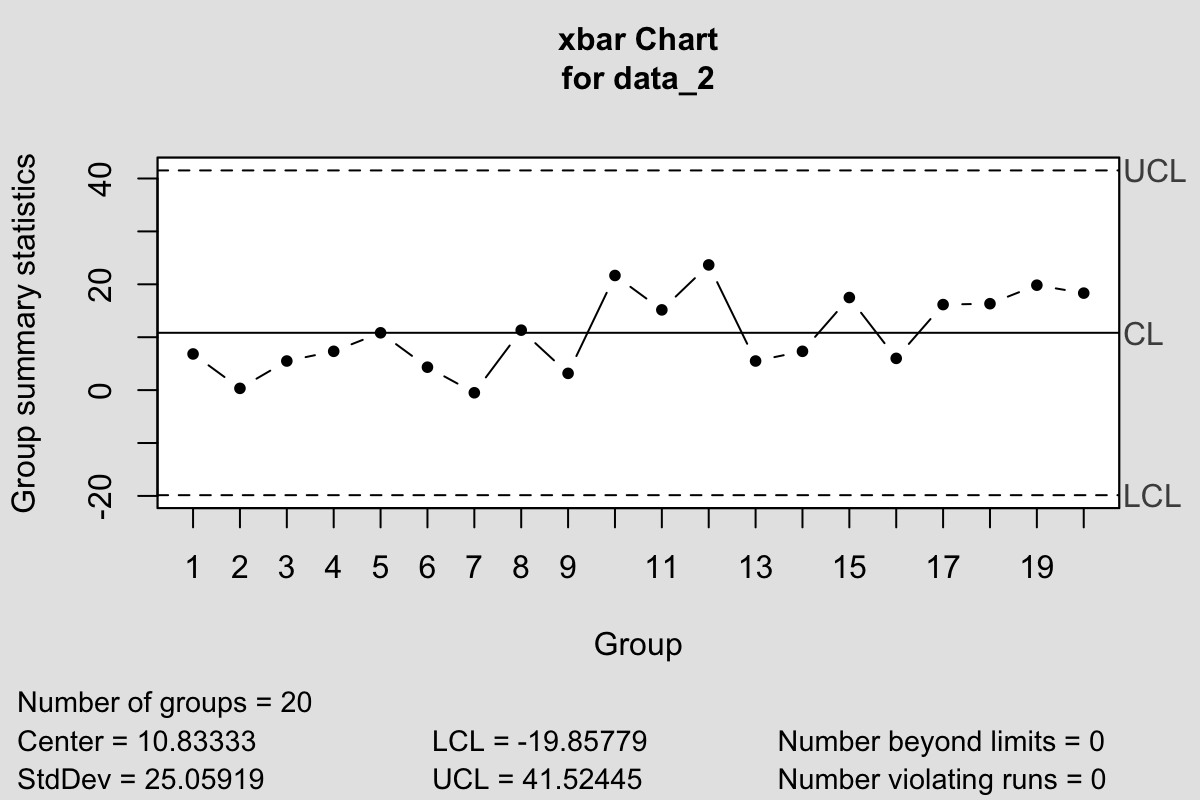
\includegraphics[width=10cm, height=7cm]{figures/Xbar_Chart_2.png}
            \caption{$\Bar{x}$ chart}
            \label{fig:3}
        \end{figure}

            
    $R$ chart:\\
    因為沒有數據在上下管制界線外,所以製程有受到控制。
        \begin{figure}[ht]
            \centering
            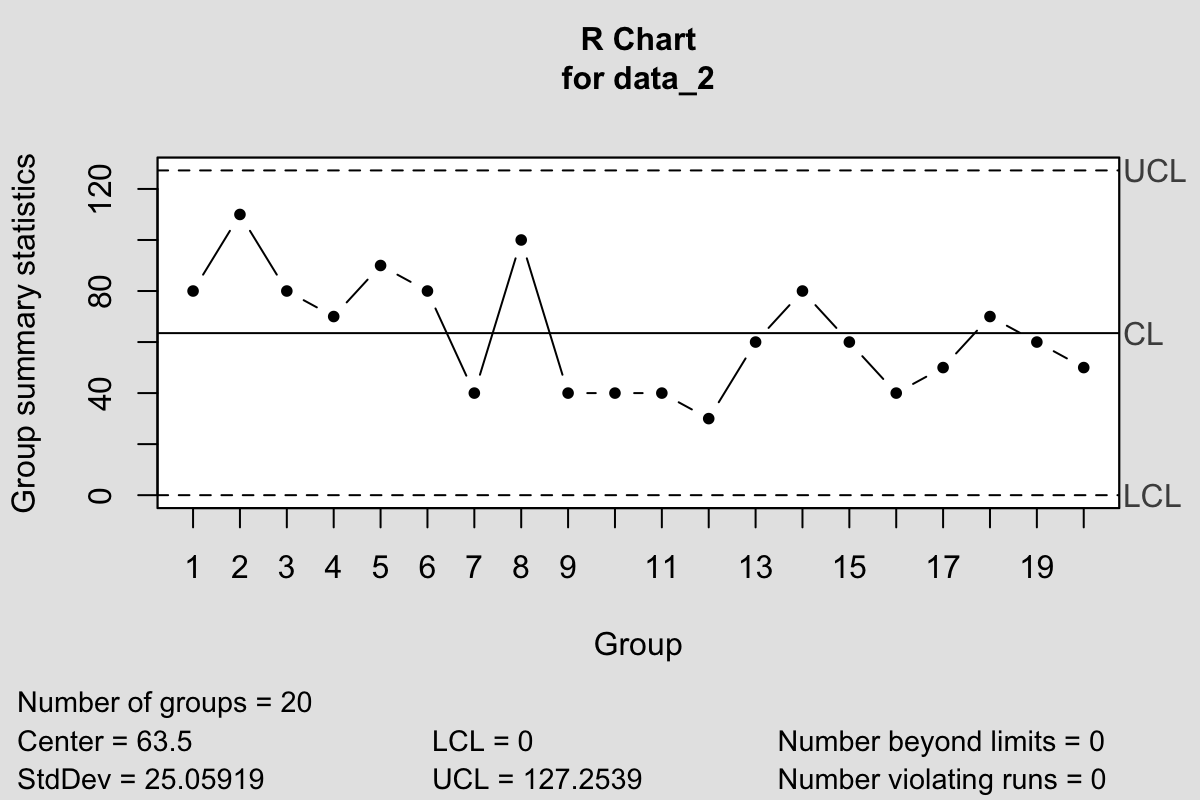
\includegraphics[width=10cm, height=7cm]{figures/R_Chart_2.png}
            \caption{$R$ chart}
            \label{fig:4}
        \end{figure}

(b) 請使用全距法估計製程標準差。
    \begin{lstlisting}[language=R]
        > ranges <- apply(data_2[, -1], 1, 
            function(row) diff(range(row)))
        > average_range <- sum(ranges) / 20
        > d2 <- 2.326
        > d3 <- 0.864
        > sigma_process_estimate <- d3 * 
            (average_range / d2)
        > print(round(sigma_process_estimate, 3))
        [1] 23.587
    \end{lstlisting}
    
(c) 如果規格為名義值 $\pm$100,請問對於這個製程你有什麼看法?請計算PCR\\
    由於 PCR ($C_p$)\ > \ 1,因此可得出該製程狀態穩定,能偵測到不良品的機率低。
    \begin{lstlisting}[language=R]
        > PCR <- 200 / (6 * sigma_process_estimate)
        > print(round(PCR, 3))
        [1] 1.413
    \end{lstlisting}
